\documentclass[12pt]{article}

\usepackage[a4paper]{geometry} %page size
\usepackage{parskip} %no paragraph indentation
\usepackage{fancyhdr} %fancy stuff in page header
\pagestyle{fancy} 

\usepackage[utf8]{inputenc} %encoding
\usepackage[danish]{babel} %danish letters

\usepackage{graphicx} %import pictures
\graphicspath{ {images/} }
\usepackage{listings} %make lists

\usepackage{amsmath, amssymb, amsfonts, amsthm, mathtools} %doing math
\usepackage{algorithmicx, algpseudocode} %doing pseudocode

\title{
  Title\
  \large Subtitle
}
\author{Asger Andersen}
\date{\today}

\fancyhead{}
\lhead{Miniprojekt 3}
\rhead{Asger Andersen}

%End of preamble
%*******************************************************************************

\begin{document}

\section*{Introduktion}

Min R-kode er vedlagt som appendix til projektet.

\section{Opgave 1}

\subsection{Delopgave a}

Reglen for differentiering af sammensatte funktioner giver os:
\begin{align}
\frac{du}{dt}=\frac{1}{K^\alpha}\alpha y^{\alpha-1} \frac{dy}{dt}
\end{align}
Ved at regne videre på dette udtryk får vi
\begin{align}
 \frac{du}{dt} = \frac{\alpha y^\alpha}{K^\alpha} y^{-1} \frac{dy}{dt} = \frac{\alpha \frac{y^\alpha}{K^\alpha}}{y} \frac{dy}{dt} = \frac{\alpha u}{y} \frac{dy}{dt}
\end{align}

\subsection{Delopgave b}

Fra linje (2) får vi let et udtryk for $y$ differentieret med hensyn til $t$:
\begin{align}
 \frac{dy}{dt} = \frac{y}{\alpha u} \frac{du}{dt}
\end{align}
Differentialligningen for $y$ giver os et andet udtryk for $y$ differentieret med hensyn til $t$. Vi kan altså sætte disse to udtryk lig hinanden:
\begin{align}
\frac{y}{\alpha u} \frac{du}{dt} = ry\left(1-\left(\frac{y}{K}\right)^\alpha\right)
\end{align}
hvilket er ækvivalent med
\begin{align}
 \frac{du}{dt} = \alpha r u \left(1-\left(\frac{y}{K}\right)^\alpha\right)
\end{align}
hvilket per definition af $u$ er ækvivalent med
\begin{align}
 \frac{du}{dt} = \alpha r u \left(1-u\right)
\end{align}

\subsection{Delopgave c}

Linje (6) er ækvivalent med
\begin{align}
 \frac{du}{dt} = (\alpha r) u \left(1-\frac{u}{1}\right)
\end{align}

Her har vi altså en helt normalt logistisk differentialligning med vækstrate $\alpha r$ og befolkningskapacitet $1$. Vi ved, at den fuldstændige løsning er
\begin{align}
u(t) = \frac{1}{1+c\exp(-\alpha r t)}, \quad c\in \mathbb{R}
\end{align}

\subsection{Delopgave d}

Per definition af $u$ følger, at 
\begin{align}
y = Ku^\frac{1}{\alpha}
\end{align}
Altså er
\begin{align}
y(t)=K(u(t))^\frac{1}{\alpha} = K\left(\frac{1}{1+c\exp(-\alpha r t)}\right)^\frac{1}{\alpha} = \frac{K}{(1+c\exp(-\alpha r t))^\frac{1}{\alpha}}
\end{align}

\subsection{Delopgave e}

Vi ser, at $y(t)=0$ og $y(t)=K$ begge er konstante løsninger til differentialligningen for $y$ (en konstant funktion differentieret er altid $0$):
\begin{align}
r\cdot 0 \left(1-\left(\frac{0}{K}\right)^\alpha\right) = 0 \\ \\ 
r\cdot K \left(1-\left(\frac{K}{K}\right)^\alpha\right) = r\cdot K \left(1-1\right) = 0
\end{align}
Altså er $y^* = 0$ og $y^*=K$ begge ligevægte for differentialligningen. 

Jeg vil nu bruge sætning $9$ på side 150 i kursusbogen Differentialligninger til at afgøre om ligevægtene er lokalt stabile eller ej.

Da 
\begin{align}
f(y) = ry\left(1-\left(\frac{y}{K}\right)^\alpha\right) = r\left(y- \frac{y^{\alpha+1}}{K^\alpha}\right)
\end{align}
afbilleder fra $\mathbb{R}$ til $\mathbb{R}$ er dens funktionalmatrix simpelthen blot dens afledede med hensyn til $y$:
\begin{align}
f'(y) = r\left(1- \frac{\alpha y^{\alpha}}{K^\alpha}\right) = r\left(1- \alpha \left(\frac{y}{K}\right)^\alpha \right)
\end{align}
Vi evaluerer dette udtryk i ligevægtene
\begin{align}
f'(0) = r\left(1- \alpha \left(\frac{0}{K}\right)^\alpha \right) = r \\ \\ 
f'(K) = r\left(1- \alpha \left(\frac{K}{K}\right)^\alpha \right) = -r\alpha
\end{align}
Vi kan betragte konstanterne $r$ og $-r\alpha$ som $1\times 1$ matricer. Da en $1\times 1$ matrix
\begin{align}
[a]
\end{align}
altid har $a$ som sin egenværdi, har funktionalmatricen evauleret i 0 og $K$ altså henholdsvis $r$ og $-r\alpha$ som egenværdi. Da $r$ og $\alpha$ begge er skarpt større end 0, så har funktionalmatricen evauleret i 0 og $K$ altså henholdsvis en ikke-negativ og en negativ egenværdi. Altså er $K$ en lokalt stabil ligevægt, hvorimod 0 ikke er lokalt stabil.

\section{Opgave 2}

\subsection{Delopgave a}

Her er et plot over antal smittede $N$ som funktion af dagen $t$:
\begin{center}
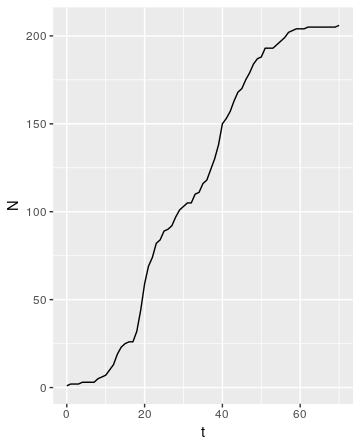
\includegraphics[scale=0.8]{q2p1.png}
\end{center}

\subsection{Delopgave b}

\begin{enumerate}
\item Den fuldstændige løsning til den logistisk differentialligning er givet som
\begin{align}
N(t) = \frac{K}{1 + c\exp(-rt)}
\end{align}
\item Ud fra de sidste målinger, sætter jeg $K=208$. Vi ved, at en logistisk funktion konvergerer mod, men aldrig når $K$. Jeg har derfor sat $K$ lidt større end de sidste målinger, da vi godt nok kan se i data, at vækstraten er aftagende, men jeg synes det virker mest rimeligt stadig at gemme lidt rum til yderligere vækst. Her er et plot, hvor $K$ er tegnet ind:
\begin{center}
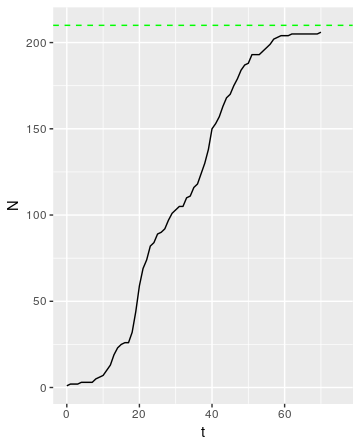
\includegraphics[scale=0.8]{q2p2.png}
\end{center}
Hermed får vi, at vores model er på formen
\begin{align}
N(t) = \frac{208}{1 + c\exp(-rt)}
\end{align}
\item Jeg antager, at $N(0)=1$, da der i dataen er 1 smittet på den 0'te dag. Hermed får vi, at 
\begin{align}
N(0) = \frac{208}{1 + c\exp(-r\cdot 0)} = \frac{208}{1 + c} = 1
\end{align}
hvilket er ækvivalent med
\begin{align}
c = 207
\end{align}
Hermed får vi, at vores model er på formen
\begin{align}
N(t) = \frac{208}{1 + 207\exp(-rt)}
\end{align}
\item Jeg plotter først nogle eksempler på modeller med $r$ mellem $0.12$ og $0.22$:
\begin{center}
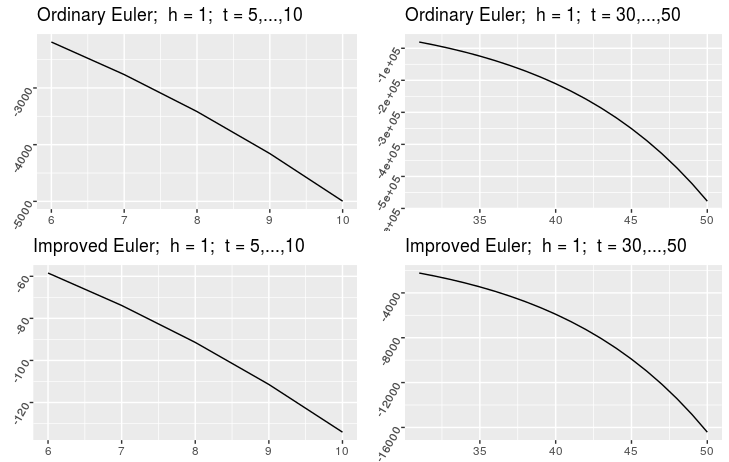
\includegraphics[scale=0.8]{q2p3.png}
\end{center}
Ud fra disse plots vælger jeg at lave nogle plots, der ser nærmere på modeller med $r$ mellem $0.14$ og $0.19$:
\begin{center}
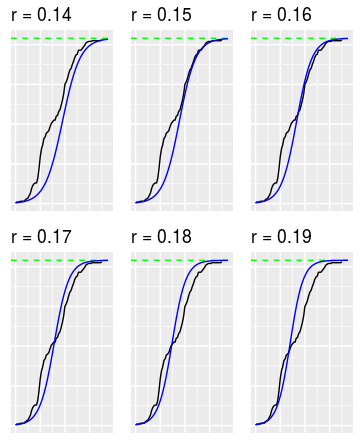
\includegraphics[scale=0.8]{q2p4.png}
\end{center}
Ud fra disse plots vælger jeg at sætte $r=0.17$, da denne model er nogenlunde præcis og desuden er den model, der ser ud til at fordele sine residualer mest ligeligt udover alle dagene.
\item Min endelige model er altså
\begin{align}
N(t) = \frac{208}{1 + 207\exp(-0.17t)}
\end{align}
En standard måde at måle hvor godt en model passer på data er summen af modellens kvadrerede residualer, hvilket i vores tilfælde er givet som
\begin{align}
S = \sum_{t=0}^{70} (N_i - N(t))^2
\end{align}
hvor $N_0, N_1, ..., N_{70}$ er de faktiske optællinger af syge på dag $0,1,...,70$. Min valgte model har $S=19549.88$. Dette tal siger dog intet som helst i sig selv uden en eller anden form for kontekst. Her er et plot af $S$ for $r=0.12,0.13,...,0.21,0.22$:
\begin{center}
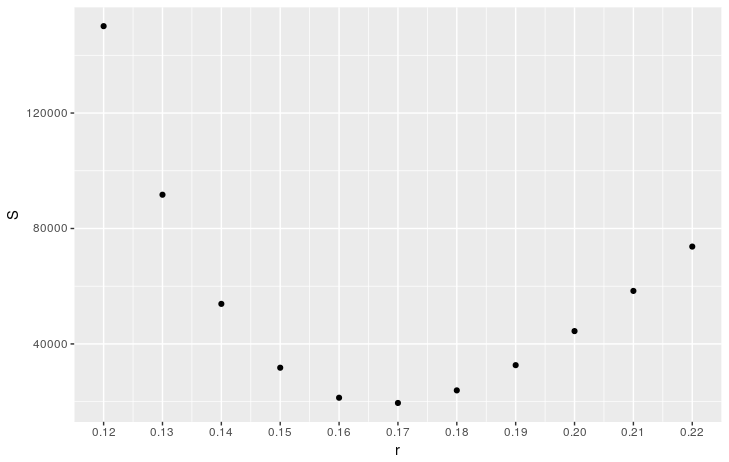
\includegraphics[scale=0.5]{q2p5.png}
\end{center}
Her ser vi, at hvis vi bruger $S$ som mål for, hvor god vores model er, så er $r=0.17$ det bedste valg ud af de testede værdier af $r$, givet mit valg af $K=208$ og $N(0)=1$.
\end{enumerate}

\subsection{Delopgave c}

\begin{enumerate}
\item Den fuldstændige løsning til den modificerede logistisk differentialligning er givet som
\begin{align}
N(t) = \frac{K}{(1+c\exp(-\alpha r t))^\frac{1}{\alpha}}
\end{align}

\item Da $\alpha, r >0$, har vi
\begin{align}
\exp(-\alpha r t) \to 0, \quad t\to \infty
\end{align}
Heraf følger, at
\begin{align}
1 + c\exp(-\alpha r t) \to 1, \quad t\to \infty
\end{align}
Heraf følger, at 
\begin{align}
(1+c\exp(-\alpha r t))^\frac{1}{\alpha} \to 1, \quad t\to \infty
\end{align}
Heraf følger, at
\begin{align}
N(t) = \frac{K}{(1+c\exp(-\alpha r t))^\frac{1}{\alpha}} \to K, \quad t\to \infty
\end{align}

Ud fra de sidste målinger, sætter jeg som ovenfor $K=208$. Hermed får vi, at vores model er på formen
\begin{align}
N(t) = \frac{208}{(1+c\exp(-\alpha r t))^\frac{1}{\alpha}}
\end{align}

\item Jeg antager, at $N(0)=1$, da der i dataen er 1 smittet på den 0'te dag. Jeg antager desuden, at $\alpha=5$. Hermed får vi, at 
\begin{align}
N(0) = \frac{208}{(1 + c\exp(-5 r\cdot 0) )^\frac{1}{5}} = \frac{208}{(1 + c)^\frac{1}{5}} = 1
\end{align}
hvilket er ækvivalent med
\begin{align}
c = 208^5 -1 = 389328928767
\end{align}
Hermed får vi, at vores model er på formen
\begin{align}
N(t) = \frac{208}{(1+389328928767\exp(-5 r t))^\frac{1}{5}}
\end{align}

Jeg plotter først nogle eksempler på modeller med $r$ mellem $0.12$ og $0.22$:
\begin{center}
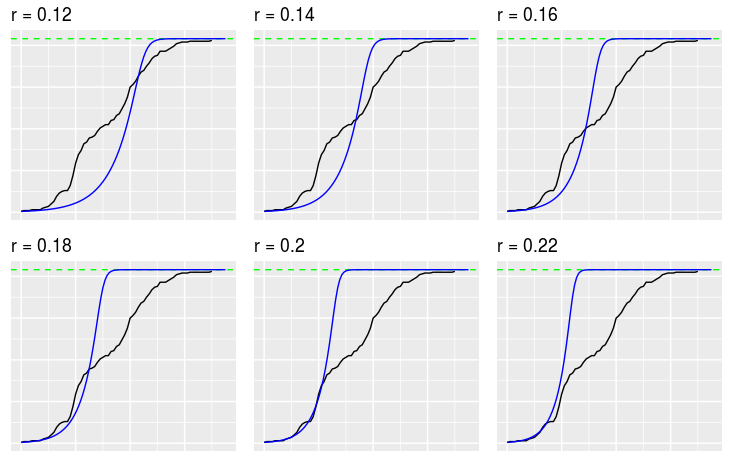
\includegraphics[scale=0.5]{q2p6.png}
\end{center}
Ud fra disse plots vælger jeg at lave nogle plots, der ser nærmere på modeller med $r$ mellem $0.12$ og $0.17$:
\begin{center}
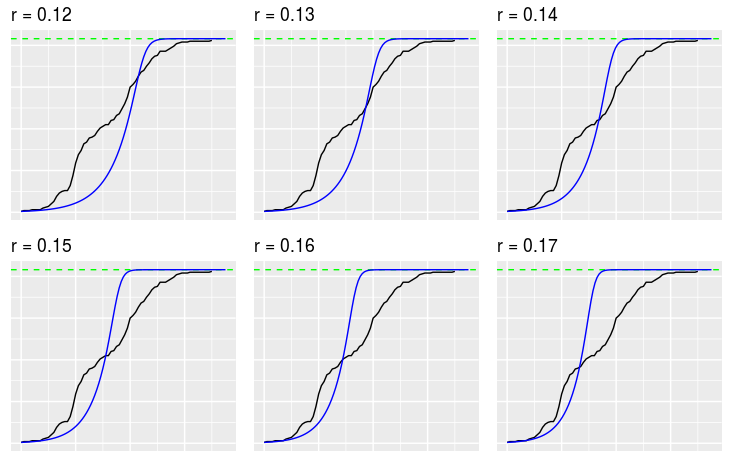
\includegraphics[scale=0.5]{q2p7.png}
\end{center}
Ud fra disse plots vælger jeg at sætte $r=0.14$.

Min endelige model er altså
\begin{align}
N(t) = \frac{208}{(1+389328928767\exp(- 0.7 t))^\frac{1}{5}}
\end{align}
Det er åbenlyst ud fra graferne, at denne model passer dårligere med data, end den simple logistiske model, jeg kom frem til i delopgave b. Her er et plot af summen af de kvadrerede residualer for $r=0.12,0.13,...,0.21,0.22$:
\begin{center}
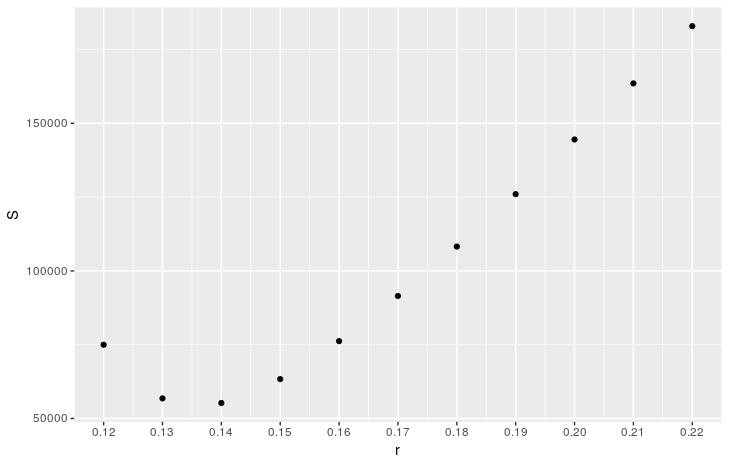
\includegraphics[scale=0.5]{q2p8.png}
\end{center}
Her ser vi, at hvis vi bruger $S$ som mål for, hvor god vores model er, så er $r=0.14$ det bedste valg ud af de testede værdier af $r$, givet valget af $K=208$, $N(0)=1$ og $\alpha=5$. Modellen har i så fald $S=55249.06$, hvilket er omtrent 2.5 gange så stort som $S$ for modellen i delopgave b. Ud fra dette kriterium er modellen fra delopgave $b$ altså også bedre.

\item Jeg antager, at $N(0)=1$, da der i dataen er 1 smittet på den 0'te dag. Jeg antager desuden, at $\alpha=0.2$. Hermed får vi, at 
\begin{align}
N(0) = \frac{208}{(1 + c\exp(-0.2 r\cdot 0) )^5} = \frac{208}{(1 + c)^5} = 1
\end{align}
hvilket er ækvivalent med
\begin{align}
c = 208^{\frac{1}{5}} -1 = 1.908
\end{align}
Hermed får vi, at vores model er på formen
\begin{align}
N(t) = \frac{208}{(1 + 1.908\exp(-0.2 r t) )^5}
\end{align}

Jeg plotter først nogle eksempler på modeller med $r$ mellem $0.38$ og $0.48$:
\begin{center}
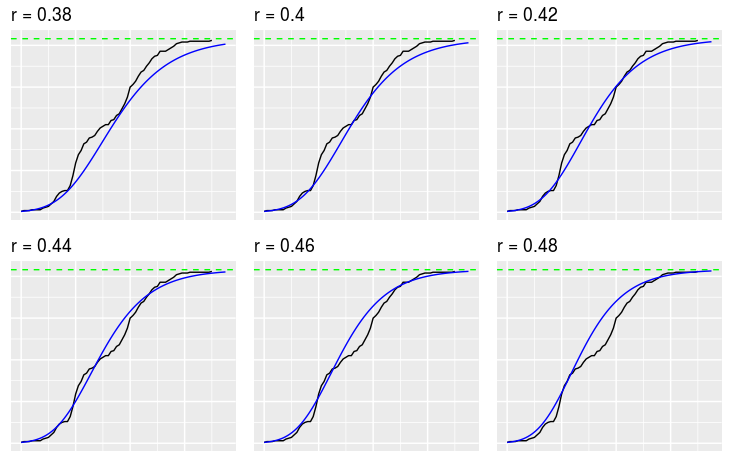
\includegraphics[scale=0.5]{q2p9.png}
\end{center}
Ud fra disse plots vælger jeg at lave nogle plots, der ser nærmere på modeller med $r$ mellem $0.4$ og $0.45$:
\begin{center}
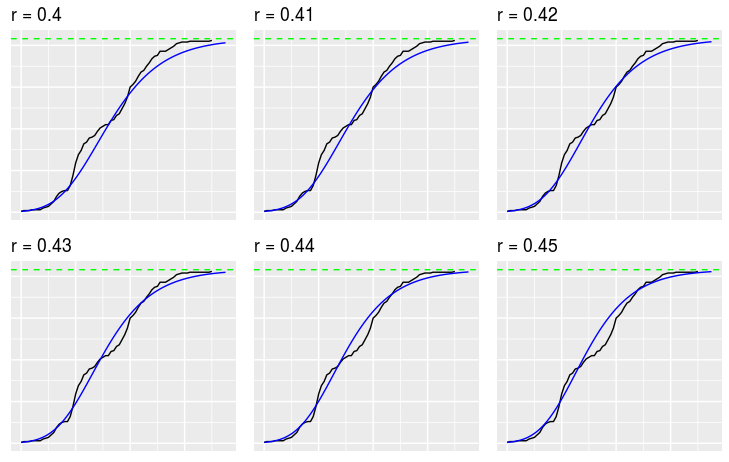
\includegraphics[scale=0.5]{q2p10.png}
\end{center}
Ud fra disse plots vælger jeg at sætte $r=0.43$.

Min endelige model er altså
\begin{align}
N(t) = \frac{208}{(1 + 1.908\exp(-0.82 t) )^5}
\end{align}
Det er ret klart ud fra graferne, at denne model passer bedre med data, end den simple logistiske model, jeg kom frem til i delopgave b. For det første er dens residualer mindre. For det andet - og lige så vigtigt - så begår den simple logistiske model en mere systematisk form for fejl, idet den konsekvent forudsiger for få antal syge i den første halvdel af epidemien og for mange syge i den sidste halvdel. I den nye model ser residualerne ud til at fordele sig mere tilfældigt omkring modellens forudsigelser (de ser dog ikke fuldstændigt tilfældige ud, men dog bedre end for den simple logistiske model).

Her er et plot af summen af de kvadrerede residualer for $r=0.38,0.39,...,0.47,0.48$ for den nye model:
\begin{center}
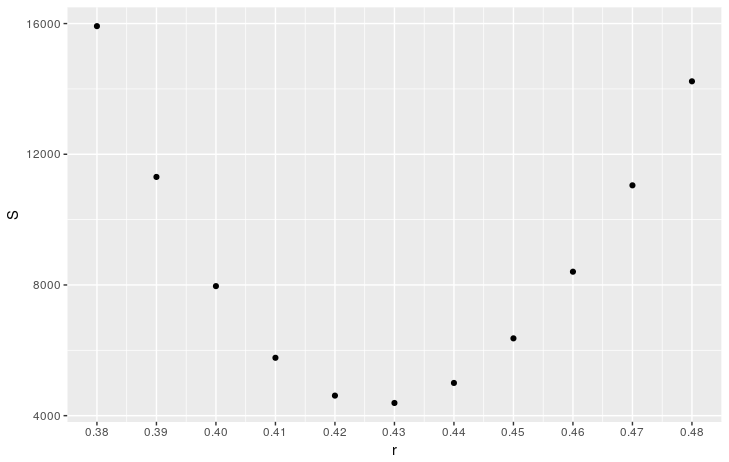
\includegraphics[scale=0.5]{q2p11.png}
\end{center}
Her ser vi, at hvis vi bruger $S$ som mål for, hvor god vores model er, så er $r=0.43$ det bedste valg ud af de testede værdier af $r$, givet valget af $K=208$, $N(0)=1$ og $\alpha=0.2$. Modellen har i så fald $S=4388.52$, hvilket er omtrent 5 gange så småt som $S$ for modellen i delopgave b. Ud fra dette kriterium er den nye model altså også bedre end modellen fra delopgave $b$.
\end{enumerate}

\subsection{Delopgave d}

\begin{enumerate}
\item Her er et plot for modellen af to kombinerede modificerede logistiske funktioner:
\begin{center}
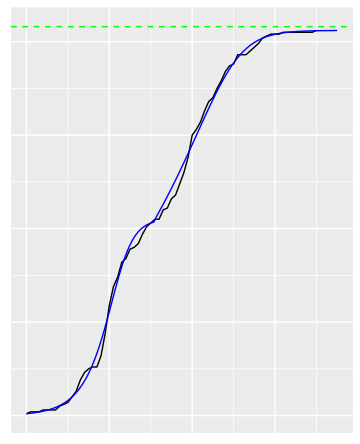
\includegraphics[scale=0.6]{q2p12.png}
\end{center}
Da $N1(31)=103.63$ og $N2(31)=105$, har funktionen $N$ ikke et særligt stort spring i $t=31$.
\item Denne model er bestemt den af vores hidtidige modeller, der passer bedst på data. Det gælder både, når vi vurderer den ud fra grafen, og når vi ser, at den har $S=667.29$, hvilket er det klart laveste hidtil. Dog ville jeg fra et metodisk perspektiv umiddelbart være skeptisk over for den måde, vi har fundet frem til modellen på. Basalt set har vi set på data, lagt mærke til et lidt mærkeligt bump og derefter konstrueret vores model ud fra dette bump. Hermed risikerer vi at overfitte til data og få en kompliceret model, der både er sværere at fortolke og har værre forudsigelseskraft på ny data, idet den har den foreliggende datas tilfældigheder bygget ind i sig.
\end{enumerate}

\section{Opgave 3}

\subsection{Delopgave a}

\subsubsection{(i)}

Vi har den inhomogene, linære 1. ordens differentialligning
\begin{align}
x'(t) = r_0x(t) - u_0 - \alpha t
\end{align}
som vi kan omskrive til  
\begin{align}
\frac{dx}{dt} + (-r_0 x) = - u_0 - \alpha t
\end{align}
hvorved den er på samme form, som kursusbogen Matematik for Biovidenskab opskriver inhomogene, linære 1. ordens differentialligninger. Hermed kan vi bruge panserformlen på side 281 til at bestemme den fuldstændige løsning til differentialligningen
\begin{align}
x(t) = \exp(-F(t)) \int \exp(F(t))g(t)\ dt  
\end{align}
hvor 
\begin{align}
F(t) = \int - r_0\ dt = -r_0t
\end{align}
og 
\begin{align}
g(t) = -u_0 -\alpha t
\end{align}
Vi har altså, at 
\begin{align}
\int \exp(F(t))g(t)\ dt = \\ 
\int \exp(-r_0t)(-u_0 -\alpha t) \ dt = \\ 
\left(-u_0\int \exp(-r_0t) \ dt\right) + \left( - \alpha \int \exp(-r_0t) t \ dt\right) = \\
\left(-u_0 \frac{-1}{r_0} \exp (-r_0t) \right) + \left( - \alpha \frac{-\exp(-r_0t)(r_0t+1)}{r_0^2}\right) + C = \\
\left(\frac{r_0u_0 + \alpha}{r_0^2} + \frac{\alpha }{r_0}t \right)\exp(-r_0t) + C  = \\
h(t)\exp(-r_0t) + C  
\end{align}
hvor 
\begin{align}
h(t) = \frac{r_0u_0 + \alpha}{r_0^2} + \frac{\alpha }{r_0}t 
\end{align}
og
\begin{align}
C \in \mathbb{R}
\end{align}

Altså har vi alt i alt nu, at den fuldstændige løsning er givet ved 
\begin{align}
x(t) = \\ 
\exp(-F(t)) \int \exp(F(t))g(t)\ dt = \\ 
\exp(r_0t) \bigg( h(t)\exp(-r_0t) + C  \bigg) = \\
h(t) + C\exp(r_0t)
\end{align}

\subsubsection{(ii)}

Vi har, at
\begin{align}
x(0) = h(0) + C\exp(r_0\cdot 0) = h(0) + C
\end{align}
hvilket giver, at
\begin{align}
C = x(0) - h(0)
\end{align}

Altså kan vi også skrive den fuldstændige løsning som
\begin{align}
x(t) = \\ h(t) + (x(0) - h(0))\exp(r_0t) = \\ h(t) + \left(x(0) - \frac{r_0u_0 + \alpha}{r_0^2}\right)\exp(r_0t)
\end{align}

\subsubsection{(iii)}

Vi ser, at 
\begin{align}
h(t) = \frac{r_0u_0 + \alpha}{r_0^2} + \frac{\alpha }{r_0}t 
\end{align}
er en linær funktion af $t$. Desuden er den voksende, da $\alpha$ og $r_0$ begge er skarpt positive. Altså går $h$ mod uendelig, når $t$ går mod uendelig. Hvis $C = 0$, så går
\begin{align}
x(t) = h(t) + C\exp(r_0 t)
\end{align}
altså mod uendelig, når $t$ går mod uendelig. Vi ved desuden, at hvis $C\neq 0$, så
\begin{align}
\frac{h(t)}{C\exp(r_0t)} \to 0, \qquad t\to \infty
\end{align}
da en eksponentiel funtion med positiv rate dominerer enhver linær funktion i det lange løb. Hvis $C\neq 0$, så har vi altså, at $x(t)$ går i minus på lang sigt, hvis og kun hvis $C<0$. Altså har vi alt i alt, at $x(t)$ undgår at gå i minus på lang sigt, hvis og kun hvis $0 \leq C$, hvilket gælder, hvis og kun hvis
\begin{align}
h(0) \leq x(0)
\end{align}
Altså har vi, at
\begin{align}
x_{\min} = h(0) = \frac{r_0u_0 + \alpha}{r_0^2}
\end{align}

\subsubsection{(iv)}

Her er mine plots:
\begin{center}
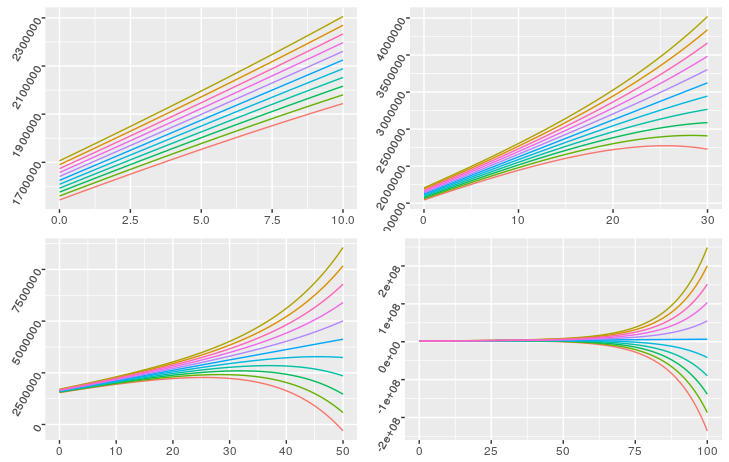
\includegraphics[scale=0.5]{q3p1.png}
\end{center}
Hvert plot viser $x(t)$ for $x_0=0.95x_{\min}, 0.96x_{\min}, ..., x_{\min}, ..., 1.04x_{\min}, 1.05x_{\min}$. Plottene adskiller sig ved at vise funktionernes udvikling for højere og højere $t$. Vi ser, at hvor alle funktionerne ser ret linære ud og følges nogenlunde ad for $t=0,...,10$, så bliver de mere og mere eksponentielle og adskiller de sig mere og mere fra hinanden jo større $t$ bliver.

\subsubsection{(iv \& v)}

Her er nogle plots af numeriske approksimationer af $x(t)$ ved hjælp af Eulers og Eulers forbedrede metode sammenlignet med den sande $x(t)$. I hvert plot er den blå linje den sande $x(t)$ og den røde linje er den numeriske approksimation:

\begin{center}
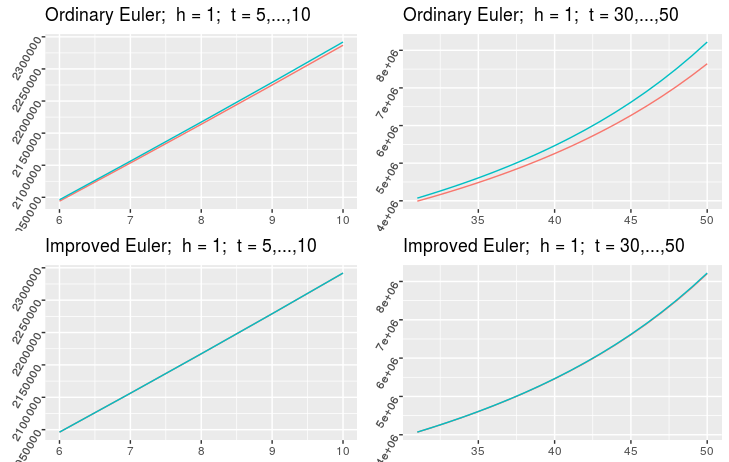
\includegraphics[scale=0.5]{q3p2.png}
\end{center}

I alle plottene er $h=1$, men vi ser på forskellige intervaller af $t$. Generelt ser vi, at Eulers forberede metode virkelig ser ud til at præstere meget bedre - faktisk i så høj grad, at grafen for den sande $x(t)$ ender med at ligge ovenpå grafen for den numeriske approksimation. Vi ser også, at de numeriske approksimationer underestimeterer den sande funktion, hvilket er forventeligt, da den sande funktion er konveks.

Her er nogle plots af, hvor store fejl de numeriske approksimationer hver især begår (fejlen er udregnet som approksimerede værdi af $x(t)$ minus den sande værdi af $x(t)$):

\begin{center}
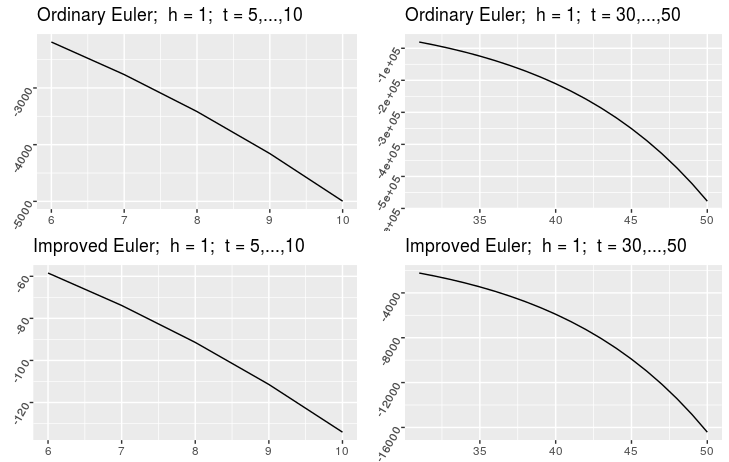
\includegraphics[scale=0.5]{q3p3.png}
\end{center}

Fejlene er negative, da approksimationerne som sagt underestimeterer den sande værdi. Vi ser, at for $t=10$ har Eulers normale metode en fejl på omkring $-5000$, mens den forbedrede metode har en fejl på omkring $-130$. Her er nogle plots, der viser, at hvis vi skal begrænse den absolutte værdi af fejlen for $t=10$ til $100$, så er det i hvert fald nok at sætte $h=0.01$ for den normale og $h=0.5$ for den forbedrede metode:
\begin{center}
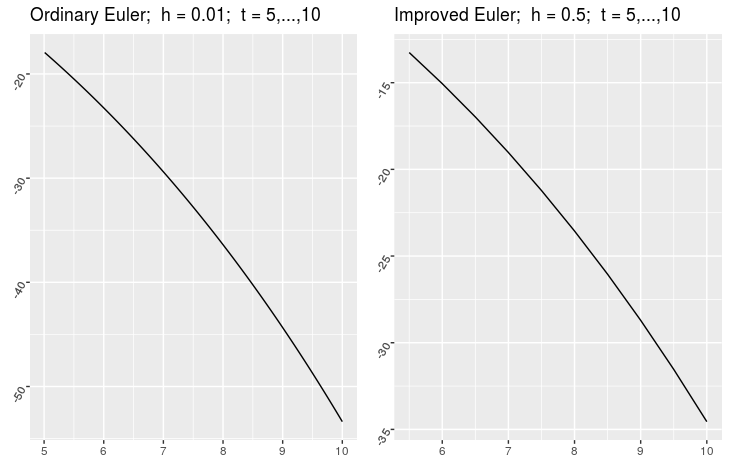
\includegraphics[scale=0.5]{q3p4.png}
\end{center}
Ved hjælp af uniroot bestemmer jeg, at for $h=0.0188$, så er fejlen $-100$ for $t=10$ for den normale metode. Ligeledes bestemmer jeg, at for $h=0.847$, så er fejlen $-100$ for $t=10$ for den forberedrede metode. 

\subsection{Delopgave b}

\subsubsection{(i)}

Vi har den inhomogene, linære 1. ordens differentialligning
\begin{align}
x'(t) = r_0x(t) - u_0\exp(\beta t)
\end{align}
som vi kan omskrive til  
\begin{align}
\frac{dx}{dt} + (-r_0 x) = - u_0\exp(\beta t)
\end{align}
hvorved den er på samme form, som kursusbogen Matematik for Biovidenskab opskriver inhomogene, linære 1. ordens differentialligninger. Hermed kan vi, som i delopgave a, løse den med panserformlen. Jeg springer mellemregningerne over og giver den fuldstændige løsning, som vi hermed kommer frem til:
\begin{align}
x(t) = j(t) + C \exp(r_0 t )
\end{align}
hvor 
\begin{align}
j(t) = \frac{u_0 }{r - \beta} \exp(\beta t)
\end{align}
og 
\begin{align}
C \in \mathbb{R}
\end{align}

\subsubsection{(ii)}

Vi har, at
\begin{align}
x(0) = j(0) + C\exp(r_0\cdot 0) = j(0) + C
\end{align}
hvilket giver, at
\begin{align}
C = x(0) - j(0)
\end{align}

Altså kan vi også skrive den fuldstændige løsning som
\begin{align}
x(t) = \\ j(t) + (x(0) - j(0))\exp(r_0t) = \\ j(t) + \left(x(0) - \frac{u_0 }{r_0 - \beta} \right)\exp(r_0t)
\end{align}

\subsubsection{(iii)}

Vi ser, at 
\begin{align}
j(t) = \frac{u_0 }{r - \beta} \exp(\beta t)
\end{align}
er en eksponentiel funktion af $t$. Altså er $x(t)$ en sum af to eksponentielle funktioner. Det gælder generelt om to eksponentielle funktioner $a \exp(\gamma t)$ pg $b \exp(\kappa t)$, at hvis $\gamma > \kappa$, så
\begin{align}
\frac{a \exp(\gamma t)}{b\exp(\kappa t)} \to 0, \qquad t\to \infty
\end{align}
Hvis vi antager, at $\beta > r$, har vi altså, at $j(t)$ dominerer udtrykket for $x(t)$, når $t$ går mod uendelig, og $j(t)$ er en eksponentiel funktion med negativt fortegn. Altså vil $j(t)$ og dermed $x(t)$ gå mod minus uendelig, når $t$ går mod uendelig. 

Hvis vi derimod antager, at $r > \beta$, så går
\begin{align}
x(t) = j(t) + (x(0) - j(0))\exp(r_0t)
\end{align}
mod uendelig, hvis $j(0) \leq x(0)$, og $x(t)$ går mod minus uendelig, hvis $x(0) < j(0)$. Altså har vi, at
\begin{align}
x_{\min} = j(0) = \frac{u_0 }{r_0 - \beta}
\end{align}

\subsubsection{(iv)}

Her er mine plots for delspørgsmål (A):
\begin{center}
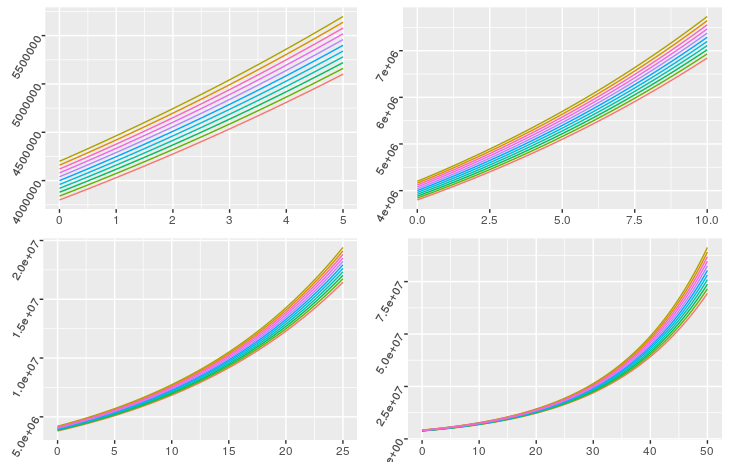
\includegraphics[scale=0.5]{q3p5.png}
\end{center}

Her er mine plots for delspørgsmål (B):
\begin{center}
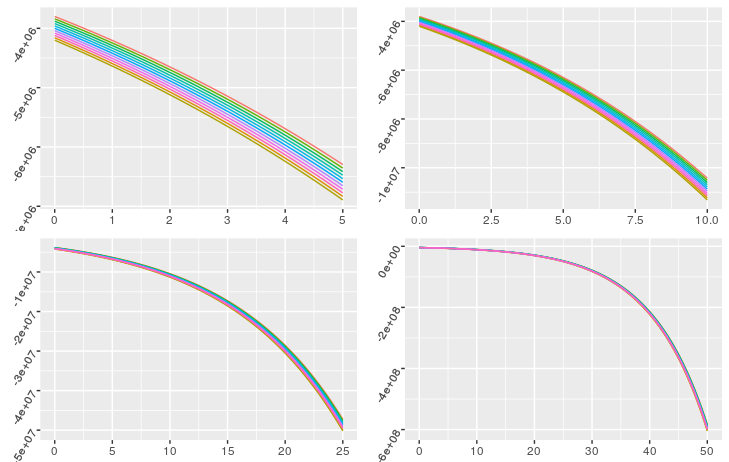
\includegraphics[scale=0.5]{q3p6.png}
\end{center}

\end{document}

